
\tikzset{every picture/.style={line width=0.75pt}} %set default line width to 0.75pt        

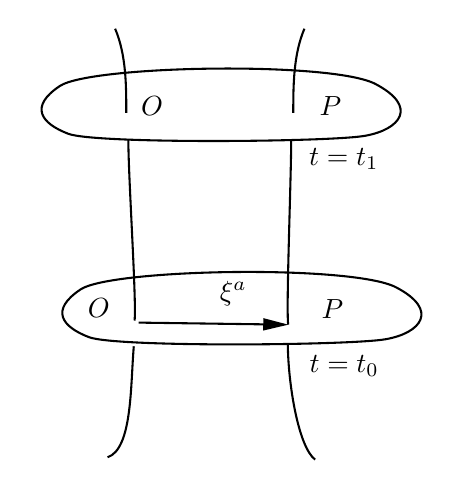
\begin{tikzpicture}[x=0.75pt,y=0.75pt,yscale=-1,xscale=1]
	%uncomment if require: \path (0,234); %set diagram left start at 0, and has height of 234
	
	%Shape: Polygon Curved [id:ds22637236277951622] 
	\draw   (247.37,40.6) .. controls (262.37,30.6) and (378.37,28.6) .. (399.37,39.6) .. controls (420.37,50.6) and (411.37,61.6) .. (394.37,64.6) .. controls (377.37,67.6) and (264.37,68.6) .. (251.37,63.6) .. controls (238.37,58.6) and (232.37,50.6) .. (247.37,40.6) -- cycle ;
	%Curve Lines [id:da18689240443569588] 
	\draw    (274,13) .. controls (279.37,25.6) and (279.37,40.6) .. (279.37,53.6) ;
	%Curve Lines [id:da17346503975046823] 
	\draw    (280.37,66.6) .. controls (280.37,84.6) and (284.37,144.6) .. (283.37,153.6) ;
	%Shape: Polygon Curved [id:ds6361529811634252] 
	\draw   (257.37,138.6) .. controls (272.37,128.6) and (388.37,126.6) .. (409.37,137.6) .. controls (430.37,148.6) and (421.37,159.6) .. (404.37,162.6) .. controls (387.37,165.6) and (274.37,166.6) .. (261.37,161.6) .. controls (248.37,156.6) and (242.37,148.6) .. (257.37,138.6) -- cycle ;
	%Curve Lines [id:da06818232449983341] 
	\draw    (283,166) .. controls (281.37,184.47) and (282.37,215.47) .. (270.37,219.47) ;
	%Curve Lines [id:da734723595223542] 
	\draw    (365.2,13) .. controls (359.83,25.6) and (359.83,40.6) .. (359.83,53.6) ;
	%Curve Lines [id:da23344765681601598] 
	\draw    (358.83,66.6) .. controls (358.83,84.6) and (356.37,146.6) .. (357.37,155.6) ;
	%Curve Lines [id:da34374856442148904] 
	\draw    (357.2,165) .. controls (357.37,184.6) and (362.37,214.6) .. (370.37,220.6) ;
	%Straight Lines [id:da7895975283807535] 
	\draw    (285.37,154.6) -- (355.37,155.57) ;
	\draw [shift={(357.37,155.6)}, rotate = 180.8] [fill={rgb, 255:red, 0; green, 0; blue, 0 }  ][line width=0.08]  [draw opacity=0] (12,-3) -- (0,0) -- (12,3) -- cycle    ;
	
	% Text Node
	\draw (285,44) node [anchor=north west][inner sep=0.75pt]    {$O$};
	% Text Node
	\draw (371,44) node [anchor=north west][inner sep=0.75pt]    {$P$};
	% Text Node
	\draw (259.37,141.6) node [anchor=north west][inner sep=0.75pt]    {$O$};
	% Text Node
	\draw (372,142) node [anchor=north west][inner sep=0.75pt]    {$P$};
	% Text Node
	\draw (323,133) node [anchor=north west][inner sep=0.75pt]    {$\xi ^{a}$};
	% Text Node
	\draw (366,69) node [anchor=north west][inner sep=0.75pt]    {$t=t_{1}$};
	% Text Node
	\draw (366.2,169) node [anchor=north west][inner sep=0.75pt]    {$t=t_{0}$};
	
	
\end{tikzpicture}